% vim: ft=tex expandtab

\documentclass[12pt]{report}
\usepackage[utf8]{inputenc}
\usepackage[serbian]{babel}
\usepackage[backend=biber, style=numeric, sorting=none]{biblatex}
\usepackage{csquotes}
\usepackage[a4paper, top=20mm, bottom=20mm, left=30mm, right=15mm, headheight=10mm, headsep=5mm, footskip=9mm]{geometry}
\usepackage{fancyhdr}
\usepackage{float}
\usepackage{fontspec}
\usepackage[acronym]{glossaries}
\usepackage{graphicx}
\usepackage{hyperref}
\usepackage{titlesec}
\usepackage{ragged2e}
\usepackage{setspace}

\hypersetup{hidelinks}

\setmainfont{Times New Roman}

\tolerance=1
\emergencystretch=\maxdimen
\hyphenpenalty=10000
\hbadness=10000

\addbibresource{literature.bib}

\pagestyle{fancy}

\renewcommand{\chaptermark}[1]{\markboth{#1}{}}
\renewcommand{\sectionmark}[1]{\markright{\arabic{section}.\ #1}}
\renewcommand{\baselinestretch}{1.4}
\newcommand{\normal}{
\tolerance=1
\emergencystretch=\maxdimen
}

\makeatletter
\newcommand\frontmatter{
    \cleardoublepage{}
    \pagenumbering{Roman}
    \setlength{\parskip}{0pt}
}

\setsansfont{Arial}

\newcommand\mainmatter{
    \cleardoublepage{}
    \pagenumbering{arabic}
    \setlength{\parskip}{2mm}
    \titleformat{\chapter}{\normalfont\Large\bf\sffamily\raggedleft}{\thechapter.}{12pt}{}
}
\makeatother

\titlespacing*{\chapter}{0mm}{58mm}{10mm}
\titleformat{\chapter}{\normalfont\Large\bf\sffamily}{\thechapter.}{12pt}{}
\titleformat{\section}{\normalfont\large\bf\sffamily}{\thesection}{12pt}{}
\titleformat{\subsection}{\normalfont\bf\sffamily}{\thesubsection}{12pt}{}
\titleformat{\subsubsection}{\normalfont\bf\sffamily}{\thesubsubsection}{12pt}{}
\setcounter{secnumdepth}{4}

\fancypagestyle{plain}{}
\fancyhead[L]{}
\fancyhead[R]{\leftmark}
\fancyfoot{}
\fancyfoot[R]{\thepage}

\raggedbottom{}

\begin{document}

\frontmatter{}

\renewcommand{\MakeUppercase}[1]{#1}
\tableofcontents

\listoffigures

\chapter*{Skraćenice}
\chaptermark{Skraćenice}
\begin{tabular}{ l l }
    \textbf{API} & -- \textit{Application programming interface}, Interfejs za programiranje aplikacija \\
    \textbf{URL} & -- \textit{Application programming interface}, Interfejs za programiranje aplikacija \\
\end{tabular}

\mainmatter{}
\chapter{Uvod}
U današnje vreme

\begin{figure}[H]
    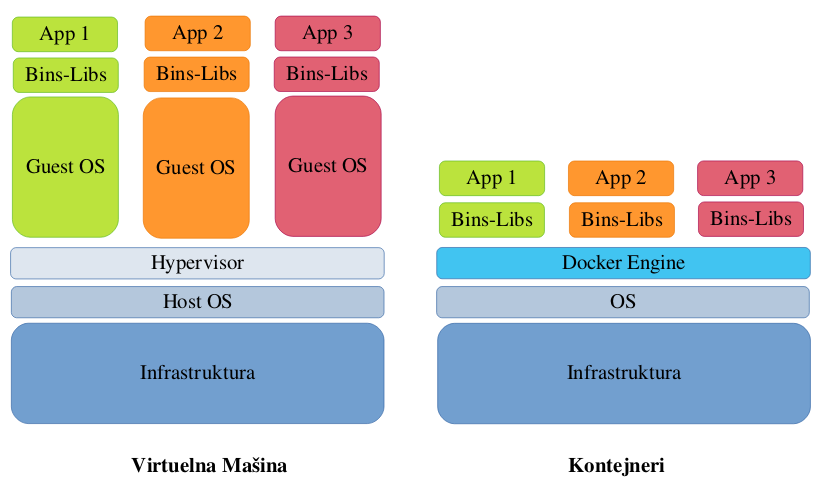
\includegraphics[width=\linewidth]{images/vm.png}
    \caption{Razlika između arhitekture Virtuelne Mašine a arhitekture kontejnera}
\end{figure}

\chapter{Teorijske osnove}
U ovom poglavlju će biti ukratko objašnjeni svi koncepti i alati koji su bili potrebni za izradu projekta o kojem ovaj rad govori. NABROJ
\section{Open source razvoj}
\section{Sistem za praćenje verzija datoteka}
Sistem za praćenje verzija datoteka (eng.\ \textit{version control system}) je sistem zadužen za praćenje istorije promena u datotekama. Promena koja se pamti se najčešće naziva revizija. Sve promene se uglavnom čuvaju na centralizovanom sistemu za skladištenje podataka i svi korisnici sa potrebnim privilegijama mogu da mu pristupaju, preuzmu najnoviju verziju datoteke ili grupe datoteka, izmene ih i zatim objave novu verziju koja se od tog momenta smatra najnovijom.

Pored najnovije verzije, čuva se i celokupna istorija promena i moguće je vratiti datoteke u bilo koju od prethodnih revizija. U poglegu softvera (eng.\ \textit{software}), ovo nam omogućava da vratimo u upotrebu bilo koju prethodnu verziju, u slučaju da dođe do greške u nekoj od novijih verzija. Istorija se čuvaju u strukturi tipa grafa:

\begin{figure}[H]
    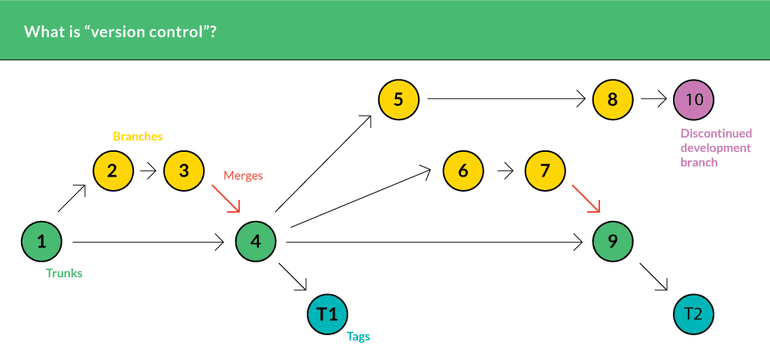
\includegraphics[width=\linewidth]{images/version.png}
    \caption{napravi novu sliku}
\end{figure}

Graf se najčešće sastoji od glavne grane(eng.\ \textit{branch}), na kojoj se nalaze glavne izmene, i pomoćnih grana na kojima se nalaze izmene za koje još nije odlučeno da li će pripadati glavnoj grani. Ako sve izmene na pomoćnim granama budu odgovarajuće, one se spajaju (eng.\ \textit{merge}) sa glavnom granom i postaju deo njenog sadržaja. U slučaju praćenja verzija softvera, ovakve grane najčešće predstavljaju nove funkcionalnosti (eng.\ \textit{feature}) koje se dodaju na glavnu granu projekta ili ispravljanje greške (eng.\ \textit{bugfix}) koja je nastala u nekoj od prethodnih verzija.

Važne izmene se mogu dodatno naglasiti dodavanjem oznake (eng.\ \textit{tag}). One uglavnom predstavljaju objavljivanje nove verzije softvera (eng.\ \textit{release}), dodavanje nove funkcionalnosti ili ispravku greške.

\section{Git}
Git \cite{git} je besplatan softver otvorenog koda (eng.\ \textit{open-source}) za praćenje verzija datoteka u distribuiranom okruženju. Primarno se koristi za razvoj softvera, ali se može koristiti i za praćenje bilo kojih drugih datoteka. Razvoj je započeo 2005. godine kreator Linux-a, Linus Torvalds, za potrebe razvoja jezgra Linux operativnog sistema. Distribuiran je pod GNU General Public License Version 2 licencom. Primarno je napravljen za Linux operativni sistem, ali je naknadno prilagođen i za macOS, BSD, Solaris i Windows.

Za razliku od drugih sistema za praćenje verzija datoteka u distribuiranom okruženju, Git nije softver klijent-server arhitekture. Svaki Git repozitorijum na svakom računaru čuva kompletnu istoriju promena i verzija i nije zavisan od pristupa mreži ili centralizovanom serveru. Kao takav, Git je osnova za razvoj mnogih drugih nezavisnih alata za praćenje verzija datoteka.

\section{GitHub}
GitHub \cite{github} je servis otvorenog koda za hostovanje (eng.\ \textit{hosting}) repozitorijuma sa različitim datotekama, najčešće izvornim kodovima za razna softverska rešenja. Za praćenje verzija datoteka, GitHub koristi Git. GitHub služi kao centralizovano mesto na kojem se čuvaju i razmenjuju sve izmene koje su sačuvane upotrebom Git alata.

U ovom trenutku, GitHub se smatra najpopularnijim alatom ovog tipa i trenutno broji preko 40 miliona korisnika. Stvari koje ovaj servis omogućava su:

\begin{enumerate}
    \item Upravljanje projektima
    \item Upravljanje timom
    \item Pregled i komentarisanje koda
    \item Integracija
    \item Akcije
    \item Paketi
    \item Bezbednost
    \item Hostovanje
\end{enumerate}

\subsection{Upravljanje projektima}
Upravljanje projektom je proces koji je potreban u bilo kojem većem programerskom projektu. Menadžeri projekta su zaduženi da prate razvoj projekta i upućuju programere u razvoj narednih delova projekata, kao i da upravljaju raspoređivanjem vremena rada na različitim zadacima koje projekat iziskuje.

GitHub nudi mogućnost koridinacije projektom, praćenje razvoja i menjanje statusa projekta na jednom mestu. Kordinacija započinje kreiranjem zadataka (eng.\ \textit{tasks}) koji traže izmene koda ili unapređenja projekta. Zadaci mogu biti u obliku greške (eng.\ \textit{issue}), komentara (eng.\ \textit{comment}) ili pull-request-a, što podrazumeva kreiranje celine koja je spremna za spajanje sa glavnom granom na projektu. Zadacima se dodeljuju osobe koje su zadužene za njih. Time će oni dobijati obaveštenja kada dođe do bilo koje izmene u kodu vezane za njihov deo posla. Zadacima je moguće dodeliti i prioritet i oznake, što dodatno olakšava proces upravljanja projektom.

Sve ove informacije moguće je pratiti i menjati u formi tabele (eng.\ \textit{board}) ili u repozitorijumu na kojem se projekat nalazi. Svaki zadatak ima unikatan URL na kojem se mogu videti sve potrebne informacije vezane za njega. Čuva se i istorija svih zadataka i izmena na projektu, kojima se stvara uvid u proces razvoja projekta. Po završetku svih zadataka, urpavljanje projektom se završava i projekat se označava kao završen.

\subsection{Upravljanje timom}
Kako u timu imamo različite uloge, koje imaju različite permisije, GitHub nudi mogućnost hijerarhijskog organizovanja učesnika na projektu gde se svakoj grupi učesnika ili pojedincu dodeljuju potrebna prava.

Takođe, moguće je dodati u repozitorijum dokumente koji se tiču projekta, kao što su kodeks ponašanja (eng.\ \textit{code of conduct}) i licenca (eng.\ \textit{license}). Ove dokumente nije potrebno svaki put pisati iznova, već postoje unapred predefinisane verzije često korišćenih kodeksa ponašanja i licenci.

\subsection{Pregled i komentarisanje koda}
Komunikacija između učesnika na projektu doprinosi kvalitetu izrade samog projekta. Pored podele zadataka i raspoređivanja vremena za svaki zadatak, javlja se potreba i za diskutovanjem koda koji se dodaje u obliku pull-request-a.

Pri kreiranju pull-request-a, GitHub nudi prikaz svih izmena u odnosu na granu sa koje su izmene krenule i na koju bi se dodale ako je sve u redu. Taj prikaz je dostupan svima koji učestvuju u izradi projekta. Moguće je, dodatno, zamoliti nekoga od učesnika da pregleda izmene pre njihovog spajanja sa odabranom granom (eng.\ \textit{requests a review}). Na svakoj od izmena, moguće je dodati poruku, koja otvara mogućnost diskusije sa ostalim učesnicima projekta. Po zavšetku, osoba koja je zadužena da pregleda izmene može da odobri ili dobije pull-request, uz mogućnost traženja dodatnih izmena pre odobrenja.

Takođe, pri kreiranju pull-request-a, GitHub automatski pregleda kod u potrazi za bezbednosnim propustima ili konfliktima sa granom sa kojom se trenutna grana spaja. Ako ih ima, GitHub obaveštava korisnika i traži izmenu pre odobrenja i spajanja koda.

\subsection{Integracija}
Pored samog pisanja aplikacije, često se javlja potreba za testiranjem i pracenjem (eng.\ \textit{monitoring}) aplikacije, automatizovanim postavljanjem u produkciju (eng.\ \textit{deployment}), kontinualnom integracijom (eng.\ \textit{continuous integration}), proverom kvaliteta koda (eng.\ \textit{code quality}) i drugim pomocnim aktivnostima u procesu razvoja softver-a.

Pošto GitHub nije u mogućnosti da ponudi sve te aktivnosti, omogućio je proces integracije sa servisima koji ih nude. Svi ovi servisi mogu se pronaći u GitHub prodavnici (eng.\ \textit{marketplace}) \cite{marketplace}. Jedna od novina u GitHub prodavnici su GitHub akcije koje će biti jedna od centralnih tema ovog rada, a bice opisane u narednoj sekciji.

\subsection{Akcije}

\subsection{Paketi}
Alati poput NPM-a, Docker-a, Maven-a, Gradle-a i drugih omogućavaju kreiranje artifakta koji sadrže sve potrebne alate za pokretanje nekog softverskog rešenja. Većina ovakvih servisa ima mogućnost čuvanja artifakta na njihovim repozitorijumima.

Zbog jednostavnosti korišćenja, GitHub je kreirao alat koji objedinjuje mnoge ovakve repozitorijume u jedan repozitorijum - GitHub Packages.

\subsection{Bezbednost}
Bezbednost u softverskim rešenjima igra veoma bitnu ulogu i najčešće zavisi od mnogo faktora: programera, ljudi koji održavaju kod (eng.\ \textit{maintainers}), istraživača, timova specijalizovanih za bezbednost i drugih. Da bi se postigao što veći stepen bezbednosti, potrebno je da što više različitih strana učestvuje u testiranju koda na bezbednosne propuste (eng.\ \textit{vulnerabilities}).

Neke od mogućnosti koje GitHub nudi za poboljšanje bezbednosti koda koji se nalazi na njemu su:

\begin{itemize}
    \item \textbf{Automatsko skeniranje koda} - pri dodavanju koda na repozitorijum, pokreće se automatsko skeniranje koda na poznate bezbednosne propuste i obaveštava se korisnika ako se pronađe neki od njih
    \item \textbf{Definisanje bezbednosnog procesa rada projekata otvorenog koda} - omogućava definisanje bezbednosnih polisa u okviru \textit{SECURITY.MD} datoteke u repozitorijumu u kojoj se navode sve potrebne informacije o tome koje bezbednosne probleme i na koji način treba da prijave korisnici koji ih pronađu
    \item \textbf{Diskutovanje o uticaju bezbednosnih propusta} - kada neki od korisnika prijavi bezbednosni propust ili grešku u kodu, GitHub nudi prostor za komentarisanje i razmenu mišljenja vezanih za postavljeni problem
    \item \textbf{Automatsko skeniranje zavisnosti} - slično skeniranju koda, pokreće se automatsko skeniranje zavisnosti nekog projekta - odnosno svih drugih softverskih rešenja od kojih projekat zavisi. Ako neko od njih ima bezbednosni propust, korisnik se obaveštava o tome. Ovakvi problemi često budu otklonjeni u narednoj verziji rešenja od kojeg projekat zavisi, pa GitHub često nudi promenu verzije kao rešenje ovakvog problema. Ovaj proces se nastavlja za vreme životnog ciklusa projekta, i ako se u bilo kojem momentu pronađe bezbednosni propust, automatski se kreira pull-request sa ispravkom
    \item \textbf{Pretraga kredencijala} - korisnicima se može desiti da slučajno upišu kredencijale za neki od eksternih servisa u kod projekta. Takvi kredencijali imaju specifičan oblik koji GitHub prepoznaje za preko 24 servisa i obaveštava korisnika ako ih pronađe
\end{itemize}

\subsection{Hostovanje sajtova}
Pored hostovanja repozitorijuma, što je glavna uloga GitHub-a, postoji i mogućnost hostovanja sajta pod GitHub domenom. Potrebno je napraviti repozitorijum sa nazivom \textit{username.github.io} i svi dokumenti u okviru njega će biti statički hostovani pod \textit{username.github.io} domenom.

\section{Python}

Python \cite{python} je programski jezik opšte namene, spada u grupu programskih jezika visokog nivoa i interpretira se. Dizajniran je tako da bude izrazito čitljiv, što se postiže velikom upotrebom belina (eng.\ \textit{whitespace character}). Pogodan je za razvoj različitih projekata pošto podržava više programskih paradigmi:

\begin{enumerate}
    \item Proceduralnu
    \item Objektno orijentisanu
    \item Funkcionalnu
    \item Strukturalnu paradigmu
\end{enumerate}

Takođe, prilagođen je za korišćenje u radličitim okruženjima na različitim operativnim sistemima.

Python se prvi put spominje krajem 1980-tih kao naslednik ABC programskih jezika. Dizajnirao ga je Guido van Rossum i objavio prvu verziju 1991. godine. Python 2.0, koji je izdat 2000. godine je znatno unapređenje prve verzije, koje se do skoro koristilo.  Poslednja velika revizija urađena je 2008. godine kada je nastao Python 3.0. Zbog toga što Python 3 nije u potpunosti kompatibilan sa prethodnim verzijama, podrška za Python prestala je u januru 2020. godine.

Umesto da poseduje svu svoju funkcionalnost u jezgru OS-a. Python je dizajniran tako da  bude veoma proširiv, što ga je učinilo veoma pogodnim za dodavanje programabilnih interfejsa postojećim aplikacijama.

\section{Python paketi, PyPI}

Python paketi su imenski prostori (eng.\ \textit{namespaces}) koji u sebi sadrže druge pakete i module - delove softvera koji obavljaju konkretnu funkcionalnost. Svaki paket je direktorijum koji u sebi mora imati \textit{\_\_init\_\_.py} datoteku. Ova datoteka može biti prazna, što označava da je trenutni direktorijum Python paket i da može biti korišćen kao zaseban modul. Inače, \textit{\_\_init\_\_.py} datoteka čuva kod koji služi za inicijaliciju tog paketa.

Da bi se koristile funkcionalnosti koje neki paket nudi, potrebno ga je uvezati (eng.\ \textit{import}) u projekat korišćenjem rezervisane reči \texttt{import}. Da bi se uvezao pojedinačni modul iz nekog paketa, treba naznačiti koji modul se iz kojeg paketa uvezuje korišćenjem sledećeg Python koda:

\begin{itemize}
    \item \texttt{from <package> import <module>}
\end{itemize}

\subsection{Distribuiranje Python paketa}

Glavna uloga Python paketa je distribuiranje biblioteka za Python programski jezik. Paket može da kreira bilo ko i da ga potom podeli sa ostatkom Python zajednice. Da bi paket bio dostupan, potrebno je kreirati arhivu sa svim potrebnim konfiguracijama za njega i objaviti je na nekom repozitorijumu za Python pakete.

Repozitorijumi su softverski alati za čuvanje i distribuiranje paketa. Postoje javni repozitorijumi, koji omogućavaju razmenu paketa sa bilo kim, i privatni, koji omogućavaju razmenu paketa u ograničenoj grupi korisnika koji imaju specijalne privilegije.

Najčešće korišćen javni repozitorijum je PyPI \cite{pypi}  - The Python Package Index.

\section{Poetry}
Poetry \cite{poetry} je alat otvorenog koda za kreiranje Python paketa i upravljanje paketima koje Python projekat koristi(eng.\ \textit{dependency management}). Pomaže korisnicima tako što umesto njih instalira i menja verzije  bibliotekama od kojih projekat zavisi, a koje korisnik mora pretkodno da specificira. Poetry je takođe znatno olakšao kreiranje, pakovanje i objavljivanje paketa na PyPI repozitorijumu i time omogućio lakše deljenje Python projekata sa drugim korisnicima Python programskog jezika.

Prva verzija alata objavljena je 28.02.2018. godine. Verzije programskog jezika Python koje su podržane su 2.7 i 3.4+. Ideja je da Poetry radi podjednako dobro na različitim platformama, između ostalog na Linux-u, Windows-u i OSX-u.

\subsection{Podešavanje Poetry-ja}
Za razliku od drugih Python alata za upravljanje paketima od kojih projekat zavisi, umesto pip-a - instalera za Python pakete, Poetry koristi svoj specifičan način za instalaciju. Instalator doda Poetry u korisnički direktorijum, tako da može da se koristi sa bilo kojom verzijom Python-a. Omogućena je i instalacija Poetry-ja korišćenjem pip-a, ali se ne proporučuje iz dva razloga:

\begin{enumerate}
    \item može dovesti do konflikta sa drugim sistemskim fajlovima
    \item otežava održavanje konzistentnosti pre korišćenju različitih verzija Python-a i različitih virtuelnih okruženja (eng.\ \textit{virtual environments})
\end{enumerate}

\subsection{Kreiranje Python projekta koji koristi Poetry}
Nakon isntalacije alata, moguće je kreirati projekat koji koristi Poetry za upravljanje paketima ili dodati Poetry u postojeći projekat i time kreirati virtuelno okruženje u kojem će se izvršavati naredne akcije. U oba slučaja će se kreirati \textit{pyproject.toml} datoteka koja čuva sve bitne informacije o projektu. U početku ova datoteka sadrži samo osnovne informacije o projektu:

\begin{samepage}
    \begin{verbatim}
    [tool.poetry]
    name = "poetry-demo"
    version = "0.1.0"
    description = ""
    authors = ["Name Surname <email>"]

    [tool.poetry.dependencies]
    python = "*"

    [tool.poetry.dev-dependencies]
    pytest = "^3.4"
    \end{verbatim}
\end{samepage}

Informacije o samom projektu, njegovom autoru, verziji, licenci, opisu, dokumentaciji, itd. nalaze se u prvom segmentu - \texttt{[tool.poetry]}. Informacije o paketima koje projekat koristi nalaze se u naredne dve sekcije - \texttt{[tool.poetry.dependencies]} i \texttt{[tool.poetry.dev-dependencies]}, gde se u prvoj od ove dve sekcije nalaze informacije o paketima koji se koriste u produkcionom okruženju, a u drogoj informacije o paketima koji se koriste u toku razvoja projekta. Pri instalaciji novog paketa, njegov naziv i verzija će se dopisati u jednu od ove dve sekcije, ili u obe ako je to potrebno.

Ovu datoteku je moguće ručno menjati, ali se sa njom najčešće interaguje pozivanjem poetry komandi u konzoli. Neke od tih komandi su:

\begin{itemize}
    \item \texttt{poetry add} - dodaje novi paket u \textit{pyproject.toml} datoteku
    \item \texttt{poetry remove} - briše paket iz projekta
\end{itemize}

Komande koje takođe interaguju sa \textit{pyproject.toml} datotekom, ali je ne menjaju su:

\begin{itemize}
    \item \texttt{poetry install} - instalira pakete definisane u \textit{pyproject.toml} datoteci
    \item \texttt{poetry update} - ažurira pakete u skladu sa verzijama koje pišu u \textit{pyproject.toml} datoteci
    \item \texttt{poetry lock} - zaključava pakete u prijektu
    \item \texttt{poetry check} - proverava ispravnost \textit{pyproject.toml} datoteke
\end{itemize}

Za pokretanje komandi u virtuelnom okruženju opsisanom u \textit{pyproject.toml} datoteci koristi se komanda:

\begin{itemize}
    \item \texttt{poetry run}
\end{itemize}

Za sve ostale detalje najbolje je pogledati dokumentaciju pomoću komande:

\begin{itemize}
    \item \texttt{poetry help}
\end{itemize}

\subsection{Kreiranje, pakovanje i objavljivanje Python paketa}
Da bi se Python projekat mogao objaviti, potrebno je kreirati arhivu sa svim potrebnim konfiguracijama za njega. To se postiže upotrebom komande:

\begin{itemize}
    \item \texttt{poetry build}
\end{itemize}

Nakon toga, paket je spreman za objavljivanje. U projektu se pojavi novi direktorijum sa nazivom \texttt{dist} i u njemu se nalaze dve datoteke:

\begin{enumerate}
    \item \texttt{poetry-demo-0.1.0-py2.py3-none-any.whl}
    \item \texttt{poetry-demo-0.1.0.tar.gz}
\end{enumerate}

Repozitorijum na kojem se paket objavljuje se podešava pomoću komande:

\begin{itemize}
    \item \texttt{poetry config}
\end{itemize}

Paket se objavljuje pozivanjem komande:

\begin{itemize}
    \item \texttt{poetry publish}
\end{itemize}

U tom momentu, paket postaje dostupan na izabranom repozitorijumu i svako ko ima pristup repozitorijumu može da instalira paket. Najčešće se paketi objavljuju na PyPI repozitorijumu.

\section{Bash}

\chapter{Specifikacija i implementacija projekta}
\section{pjisp-assignment-template}
\section{pjisp-template-name}
\subsection{način imenovanja repo-a}
\section{pjisp-diff}
\section{poetry-publish action}
Koristi se za publishovanje pjisp-diff i pjisp-template-name
\section{Error code u smoke-test-u - zasto je potreban?}


\chapter{Primeri korišćenja}
\chapter{Diskusija i zakljuci}
\section{Da li su github akcije spremne za produkciju?}
\chapter{Literatura}
\sloppy
\printbibliography[heading=none]

\end{document}
